\documentclass[9pt]{article}
\usepackage{graphicx}
\usepackage[utf8]{inputenc}
%\usepackage[T1]{fontenc}
\usepackage{textcomp}
%\usepackage[dutch]{babel}
\usepackage{amsmath, amssymb}

\begin{document}
\title{Fun With Pipes}
\author{Anthony Steel}
\date{\today}
\maketitle
While working on some plumping with my dad, questions related to the fluid
dynamics of pipes arose. Having never studied fluids, I thought it would be
interesting to see which equations I could derive from mechanical considerations
of the fluids in the pipes.
\section{Pipes of different radii}
Consider two cylindrical pipes of radii $r_1$ and $r_2$ connected to one another.
In them flows a fluid which is assumed to be incompressible and has density $\rho$.
Furthermore, consider a slice of the fluid of extent $x$ at two times, one
before and one after the boundary as shown in Figure $\ref{pipes}$. Consider
conservation of energy on this slice of the fluid:
\[
  \int F_1 dx + \frac{1}{2} m_1 v_1^2 + m_1 g h_1 = \int F_2 dx + \frac{1}{2} m_2 v_2^2 + m_2 g h_2
\]
Rewriting the masses in terms of the densities and volumes using $m_i = \rho V_i = \pi \rho r_i^2 x$.
\[
  \int F_1 dx + \frac{1}{2} \rho \pi r_1^2 x v_1^2  + \pi \rho r_1^2 x g h_1 = \int F_2 dx + \frac{1}{2} \pi \rho r_2^2 x v_2^2 + \pi \rho r_2^2 x g h_2
\]
\begin{figure}
  \begin{center}
  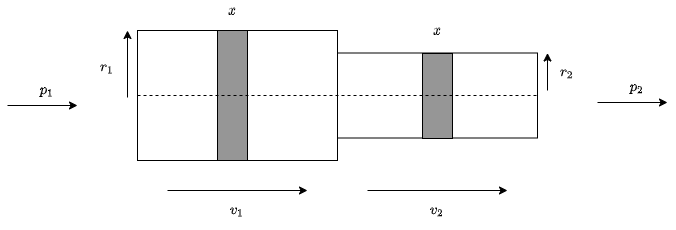
\includegraphics[width=1.0\textwidth]{images/pipes.png}
  \end{center}
  \caption{}
  \label{pipes}
\end{figure}
Write the forces in terms of the pressures using $F_i = p_i A_i = \pi p_i r_i^2$.
Assuming the pressures are constant:
\[
  \pi p_1 r_1^2 x + \frac{1}{2} \rho \pi r_1^2 x v_1^2  + \pi \rho r_1^2 x g h_1 = \pi p_2 r_2^2 x + \frac{1}{2} \pi \rho r_2^2 x v_2^2 + \pi \rho r_2^2 x g h_2
\]
\[
  p_1 r_1^2 + \frac{1}{2} \rho r_1^2 v_1^2  + \rho r_1^2 g h_1 = p_2 r_2^2 + \frac{1}{2} \rho r_2^2 v_2^2 + \rho r_2^2 g h_2
\]
\[
  r_1^2 (p_1 + \frac{1}{2} \rho v_1^2  + \rho g h_1) = r_2^2 (p_2 + \frac{1}{2} \rho v_2^2 + \rho g h_2)
\]
Consider some special cases of the above equation.
\subsection{$r_1 = r_2$}
We regain Euler's equation:
\[
  p_1 + \frac{1}{2} \rho v_1^2  + \rho g h_1 = p_2 + \frac{1}{2} \rho v_2^2 + \rho g h_2
\]
\subsection{Abscence of Gravity}
\[
  r_1^2 (p_1 + \frac{1}{2} \rho v_1^2 ) = r_2^2 (p_2 + \frac{1}{2} \rho v_2^2 )
\]
This relationship is kinematical in nature. It would be nice to know how the
fluid evolves through time.
\section{$F = ma$ for the fluid}
\[
  F = \frac{d}{dt} (m v)
\]
Rewriting in terms of pressure and density:
\[
  - p A = \frac{d}{dt} (\rho V v)
\]
\end{document}
